\documentclass[12pt,a4paper]{article}
\usepackage[utf8]{inputenc}
\usepackage[T1]{fontenc}
\usepackage[spanish,es-noshorthands]{babel}
\usepackage{geometry}
\geometry{a4paper, margin=2.5cm}
\usepackage{booktabs}
\usepackage{graphicx}
\usepackage{hyperref}
\usepackage{xcolor}
\usepackage{tabularx}
\usepackage{array}
\usepackage{listings}
\usepackage{amsmath}
\usepackage{url}

\hypersetup{
    colorlinks=true,
    linkcolor=blue,
    filecolor=magenta,      
    urlcolor=blue,
    pdftitle={¿Qué es PlatformIO? - ESP32 Kids Lab},
    pdfauthor={Laboratorio ESP32},
}

\sloppy
\emergencystretch 3em

\definecolor{codegreen}{rgb}{0,0.6,0}
\definecolor{codegray}{rgb}{0.5,0.5,0.5}
\definecolor{codepurple}{rgb}{0.58,0,0.82}
\definecolor{backcolour}{rgb}{0.96,0.96,0.96}

\lstdefinestyle{mystyle}{
    backgroundcolor=\color{backcolour},   
    commentstyle=\color{codegreen},
    keywordstyle=\color{blue},
    numberstyle=\tiny\color{codegray},
    stringstyle=\color{codepurple},
    basicstyle=\ttfamily\small,
    breakatwhitespace=false,         
    breaklines=true,                 
    captionpos=b,                    
    keepspaces=true,                 
    numbers=left,                    
    numbersep=5pt,                  
    showspaces=false,                
    showstringspaces=false,
    showtabs=false,                  
    tabsize=2,
    literate=
      {á}{{\'a}}1 {é}{{\'e}}1 {í}{{\'i}}1 {ó}{{\'o}}1 {ú}{{\'u}}1
      {Á}{{\'A}}1 {É}{{\'E}}1 {Í}{{\'I}}1 {Ó}{{\'O}}1 {Ú}{{\'U}}1
      {ñ}{{\~n}}1 {Ñ}{{\~N}}1
}

\lstset{style=mystyle}

\title{\textbf{Plataforma de Desarrollo PlatformIO:\\ Fundamentos, Arquitectura y Aplicación en ESP32 Kids Lab}}
\author{Proyecto: ESP32 Kids Lab}
\date{\today}

\begin{document}

\maketitle

\begin{abstract}
Este documento presenta una descripción técnica y conceptual de \textbf{PlatformIO}, un ecosistema profesional de código abierto para el desarrollo de sistemas embebidos e Internet de las Cosas (IoT). Se abordan sus características arquitectónicas, su sistema de gestión de dependencias, la configuración declarativa mediante el archivo \texttt{platformio.ini}, y su rol crucial dentro del proyecto educativo \textbf{ESP32 Kids Lab}.
\end{abstract}

\vspace{0.8cm}
\tableofcontents
\newpage

\section{Introducción a PlatformIO}

\textbf{PlatformIO} es un entorno de desarrollo profesional, modular y multiplataforma concebido específicamente para la ingeniería de software en microcontroladores y dispositivos IoT. Nació como una solución moderna para superar las limitaciones estructurales del entorno tradicional de Arduino IDE, proporcionando herramientas avanzadas propias de la ingeniería de software contemporánea: control de versiones riguroso, compilación declarativa, gestión aislada de librerías y depuración integrada.

A diferencia de los entornos cerrados o propietarios de cada fabricante de microchips, PlatformIO opera como una capa de abstracción universal e independiente que se integra de manera transparente en editores modernos como \textbf{Visual Studio Code}, \textbf{VSCodium}, \textbf{CLion} o directamente a través de su potente interfaz de línea de comandos (\textbf{PlatformIO Core CLI}).

\section{Pilares y Capacidades Principales}

El éxito y adopción de PlatformIO en la industria y la educación se fundamentan en seis pilares esenciales:

\subsection{1. Multiplataforma y Soporte Multi-arquitectura}
PlatformIO soporta de fábrica más de 50 plataformas de desarrollo de hardware, más de 1\,000 placas de desarrollo y los principales microcontroladores del mercado:
\begin{itemize}
    \item \textbf{Espressif Systems:} ESP32 (incluyendo familias S2, S3, C3, C6), ESP8266.
    \item \textbf{STMicroelectronics:} Familias STM32 (ARM Cortex-M).
    \item \textbf{Atmel / Microchip:} AVR (ATmega328P, ATmega2560), SAMD.
    \item \textbf{Raspberry Pi:} Microcontrolador RP2040 (Raspberry Pi Pico).
    \item \textbf{Nordic Semiconductor:} nRF51, nRF52 (Bluetooth Low Energy).
\end{itemize}

Asimismo, permite alternar entre distintos \textit{frameworks} de desarrollo para un mismo chip sin alterar el flujo de trabajo (por ejemplo, alternar entre \textbf{Arduino Core}, \textbf{ESP-IDF}, \textbf{Zephyr RTOS} o \textbf{FreeRTOS}).

\subsection{2. Gestión Inteligente y Aislada de Dependencias (\texttt{lib\_deps})}
En los entornos tradicionales, las bibliotecas se instalan globalmente en el sistema del usuario, provocando conflictos entre proyectos que requieren versiones distintas de una misma librería. PlatformIO resuelve esto mediante su registro centralizado (\textit{PlatformIO Registry}, con más de 12\,000 bibliotecas) y el aislamiento por proyecto:
\begin{itemize}
    \item Cada proyecto declara sus dependencias específicas en su archivo de configuración.
    \item Las bibliotecas se descargan automáticamente en la carpeta local \path{.pio/libdeps/}.
    \item Soporta resolución semántica de versiones (ej. \path{@^6.21.3}) o enlaces directos a repositorios Git.
    \item Garantiza que el proyecto pueda clonarse en cualquier máquina y compilar de inmediato sin instalaciones manuales previas.
\end{itemize}

\subsection{3. Configuración Declarativa (\texttt{platformio.ini})}
Toda la configuración del proyecto se define en un único archivo de texto plano: \texttt{platformio.ini}. Esto implementa la filosofía de \textit{Firmware as Code}, permitiendo que los parámetros de compilación, microcontrolador, velocidad del monitor serie, particiones de memoria flash y dependencias queden registrados bajo control de versiones Git.

\subsection{4. Sistema de Construcción Basado en SCons}
Bajo el capó, PlatformIO utiliza \textbf{SCons}, una herramienta de construcción en Python de última generación. Esto permite:
\begin{itemize}
    \item Compilación incremental y concurrente (multinúcleo), reduciendo drásticamente los tiempos de compilación.
    \item Generación de bases de datos de compilación (\path{compile_commands.json}), posibilitando autocompletado e IntelliSense con precisión de compilador real.
    \item Scripts de pre y post-procesamiento en Python para automatizar tareas (firmado de binarios, generación de cabeceras, etc.).
\end{itemize}

\subsection{5. Depuración Unificada (\textit{Unified Debugger})}
Permite depurar código paso a paso directamente sobre el hardware (empleando sondas JTAG, SWD, ESP-Prog o depuradores CMSIS-DAP) usando la misma interfaz gráfica en VS Code, con soporte de puntos de interrupción (\textit{breakpoints}), inspección de registros y memoria en tiempo real.

\subsection{6. Pruebas Unitarias Integradas (\textit{Unit Testing})}
Cuenta con el framework de pruebas unitarias \textbf{Unity}, permitiendo ejecutar pruebas automáticas tanto en el ordenador anfitrión (\textit{host testing}) como directamente en el microcontrolador conectado.

\section{Estructura de un Proyecto en PlatformIO}

Un proyecto estándar de PlatformIO presenta una jerarquía de directorios clara y estandarizada:

\begin{lstlisting}[language=bash, caption={Árbol de directorios de un proyecto PlatformIO estándar.}]
proyecto_iot/
|-- .pio/                  # Cache, objetos compilados y librerías locales
|-- .vscode/               # Configuraciones de IntelliSense para el editor
|-- include/               # Archivos de cabecera (.h, .hpp) del proyecto
|-- lib/                   # Librerías privadas o módulos locales
|-- src/                   # Código fuente C/C++ principal (ej. main.cpp)
|-- data/                  # Archivos web o datos para el sistema de archivos
|-- test/                  # Casos de prueba unitaria (Unity)
|-- platformio.ini         # Manifiesto central de configuración
\end{lstlisting}

\section{PlatformIO en el Proyecto ESP32 Kids Lab}

En el laboratorio educativo interactivo \textbf{ESP32 Kids Lab}, PlatformIO desempeña un rol neurálgico, garantizando la integración armónica entre el código C++ del ESP32 y la interfaz web servida desde la memoria flash.

\subsection{Configuración del Proyecto (\texttt{platformio.ini})}
El archivo \texttt{platformio.ini} utilizado en el proyecto ilustra el poder declarativo de PlatformIO:

\begin{lstlisting}[caption={Archivo platformio.ini de ESP32 Kids Lab.}]
[env:esp32dev]
platform = espressif32
board = esp32dev
framework = arduino
lib_ldf_mode = deep
monitor_speed = 115200
board_build.filesystem = littlefs
lib_deps = 
    https://github.com/me-no-dev/ESPAsyncWebServer.git
    https://github.com/me-no-dev/AsyncTCP.git
    bblanchon/ArduinoJson@^6.21.3
    https://github.com/avishorp/TM1637.git
    adafruit/Adafruit NeoPixel @ ^1.11.0
    paulstoffregen/OneWire @ ^2.3.7
    milesburton/DallasTemperature @ ^3.11.0
    adafruit/Adafruit GFX Library @ ^1.11.9
    adafruit/Adafruit SSD1306 @ ^2.5.9
\end{lstlisting}

\subsection{Explicación de las Claves de Configuración}
\begin{itemize}
    \item \texttt{board\_build.filesystem = littlefs}: Especifica el motor de sistema de archivos \textbf{LittleFS}, que empaqueta los archivos de la carpeta \path{data/} (\texttt{index.html}, \texttt{style.css}, \texttt{app.js}) y los transfiere a una partición reservada en la memoria Flash del ESP32.
    \item \texttt{lib\_ldf\_mode = deep}: Activa el modo de análisis profundo de dependencias (\textit{Library Dependency Finder}). Es indispensable cuando librerías asíncronas complejas como \texttt{ESPAsyncWebServer} dependen a su vez de capas de red de bajo nivel como \texttt{AsyncTCP}.
    \item \texttt{monitor\_speed = 115200}: Establece la velocidad de comunicación del puerto serie para diagnóstico y telemetría en tiempo real.
    \item \texttt{lib\_deps}: Automatiza la instalación de las 9 librerías necesarias sin que el usuario deba buscar archivos ZIP o instalar bibliotecas a mano en el sistema operativo.
\end{itemize}

\subsection{Recomendaciones de Recursos y Caché de Compilación}
Durante el proceso de compilación y enlace de proyectos complejos para el ESP32, PlatformIO descarga herramientas de cadena de montaje (\textit{toolchains}), núcleos de plataformas y dependencias en el directorio del usuario (en sistemas Windows típicamente ubicado en \path{C:\Users\<Usuario>\.platformio}). Para evitar fallos por falta de memoria (\textit{out of memory}) o saturación de almacenamiento, es aconsejable seguir pautas prácticas de optimización operativa, tal como se resume en la Figura~\ref{fig:platformio_cache}:
\begin{itemize}
    \item Cerrar instancias y navegadores innecesarios para maximizar la memoria RAM disponible antes de lanzar la compilación.
    \item Asegurar un margen amplio de espacio libre en disco (al menos 15\,GB libres recomendados para descargas de SDKs y cachés).
    \item Permitir que los procesos de compilación pesados completen su ciclo sin interrupciones forzadas, permitiendo que SCons indexe correctamente los archivos objeto.
\end{itemize}

\begin{figure}[htbp]
    \centering
    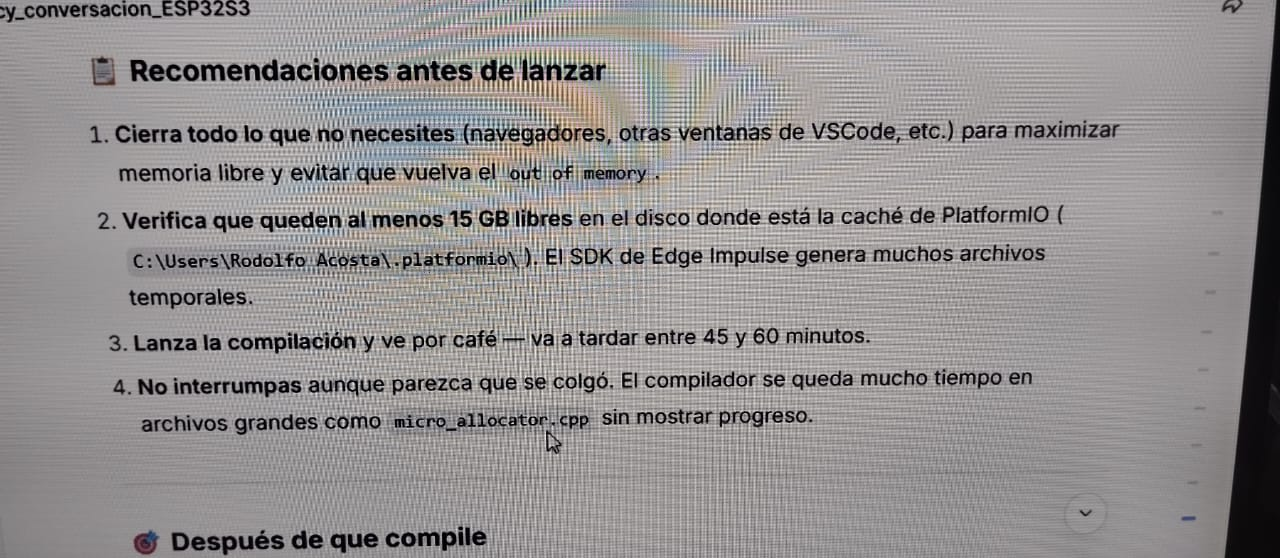
\includegraphics[width=0.75\textwidth]{platformio.jpeg}
    \caption{Recomendaciones operativas de memoria y espacio en disco para el entorno PlatformIO.}
    \label{fig:platformio_cache}
\end{figure}

\section{Comparativa Técnica: PlatformIO vs. Arduino IDE}

A continuación se comparan las diferencias clave entre el flujo de trabajo convencional y el ofrecido por PlatformIO:

\vspace{0.3cm}
\noindent
\begin{table}[htbp]
\centering
\small
\begin{tabularx}{\textwidth}{>{\bfseries\raggedright\arraybackslash}p{3cm} >{\raggedright\arraybackslash}X >{\raggedright\arraybackslash}X}
\toprule
\textbf{Criterio} & \textbf{Arduino IDE (Clásico)} & \textbf{PlatformIO} \\
\midrule
Gestión de Librerías & Global y manual; riesgo de colisiones entre versiones de proyectos. & Local por proyecto (\path{lib_deps}); versiones fijadas y deterministas. \\
\addlinespace
Configuración & Menús desplegables manuales en GUI no versionables. & Declarativa en texto (\texttt{platformio.ini}); versionable en Git. \\
\addlinespace
Editor de Código & Editor básico con herramientas limitadas de refactorización. & Integrado en VS Code con IntelliSense completo, Git y atajos avanzados. \\
\addlinespace
Sistemas de Archivos & Requiere plugins externos complejos para SPIFFS/LittleFS. & Comando nativo de subida (\texttt{uploadfs}) integrado en el flujo. \\
\addlinespace
Depuración & Casi exclusivamente por \texttt{Serial.println}. & Depuración por hardware en circuito (JTAG, GDB, Breakpoints). \\
\addlinespace
Integración CI/CD & Compleja de automatizar en servidores remotos. & Nativa y directa mediante línea de comandos (\texttt{pio run}). \\
\bottomrule
\end{tabularx}
\caption{Comparativa técnica entre Arduino IDE y PlatformIO.}
\label{tab:comparativa}
\end{table}

\section{Comandos Principales de la CLI de PlatformIO}

Aunque la mayoría de los usuarios emplean los botones gráficos de la extensión de VS Code, PlatformIO dispone de una completa suite de comandos de consola:

\begin{itemize}
    \item \texttt{pio run}: Compila el código fuente del proyecto y genera los binarios.
    \item \texttt{pio run --target upload}: Compila y descarga el firmware al microcontrolador conectado por USB.
    \item \texttt{pio run --target uploadfs}: Genera la imagen del sistema de archivos LittleFS desde la carpeta \path{data/} y la flashea en la memoria Flash.
    \item \texttt{pio device monitor}: Abre el monitor serial interactivo según la velocidad configurada.
    \item \texttt{pio lib search <nombre>}: Realiza búsquedas de bibliotecas en el registro de PlatformIO.
\end{itemize}

\section{Conclusión}

\textbf{PlatformIO} representa el estándar actual para el desarrollo profesional y robusto de sistemas embebidos. En el marco del proyecto \textbf{ESP32 Kids Lab}, su adopción no solo garantiza reproducibilidad y facilidad de despliegue en múltiples puestos de trabajo, sino que inculca en los estudiantes y desarrolladores las mejores prácticas de la ingeniería de software: modularidad, aislamiento de dependencias y reproducibilidad del firmware.

\end{document}
